\documentclass{article}	
\usepackage[a4paper, portrait, margin=1in]{geometry}
\usepackage{amsmath, graphicx, gensymb, float}
\usepackage{chngcntr}
\counterwithin{figure}{section}
\graphicspath{{./images/}}
\usepackage[utf8]{inputenc}
\usepackage{textcomp}
\usepackage{multirow}
\usepackage[english, macedonian]{babel}

\usepackage{biblatex}
\addbibresource{sample.bib}


%TO DO LIST (NOT IN ANY PARTICULAR ORDER)

%	REFERENCES
%		BIBLIOGRAPHY

%	VECTOR FIELD HISTOGRAM

%	REWORD 2ND AND 3RD PARAGRAPH IN ВОВЕД

\title{Мехатронички Системи: Управување со Повратна Врска}
\date{2.2.18}
\author{Галевски Марко 1172, Мучев Никола 1017, Наумовска Елена 1019}

\begin{document}
    \pagenumbering{gobble}
    \maketitle{}
    \newpage
    \tableofcontents
    \newpage
    \pagenumbering{arabic}
    
\section{Вовед}
Роботика и автоматика стануваат потребни и основни делови од инженерството и следствено се многу важни теми за проучување од страна на студенти на инженерство и наука. Понатаму, роботика е изградена врз темели како карактеризација на трансдусери, контрола на мотори, собирање на податоци, механика на движење, мрежна комуникација, компјутерска перцепција, препознавање на шеми, кинематика, планирање на траекторија, и други кои исто така се темели за други полиња како на пример производство. National Instruments (NI) LabVIEW комплетот за роботика заедно со LabVIEW програмскиот пакет нудат додаток на традиционалните учебници за роботика, со можност за активно/практично учење во компактен и проширлив комплет.

Проектот беше изработен со цел да го прикаже концептот и принципот позади управувањето на некој систем со повратна врска. За остварувањето на задачата употребивме еден почетен кит за роботика од National Instruments, роботот DaNI 2.0. Овој роботски кит ги содржи сите компоненти потребни за успешна реализација на задачи и проекти поврзани со управувањето и задвижувањето на еден општ робот во форма на „Rover“. 

Во текот на овој документ ќе се разговара за структурата на роботот - односно неговите сензори и актуатори, како и за управувачката единица sbRIO, исто од NI. Потоа, ќе се претставаат и образложаат 3 алгоритми во LabVIEW. Првите два ќе бидат базирани на ПИД управување со повратна врска, додека третиот алгоритам ќе биде едно детално објаснување на почетната програмата дадена од NI како пример за можните способности на DaNI. За крај, ќе се продискутира за некои предизвици со кои се соочивме во текот на изработката на овој проект, и ќе се разговара за понатамошна работа со DaNI за постигнување на некоја корисна функција.

\begin{figure}[H]
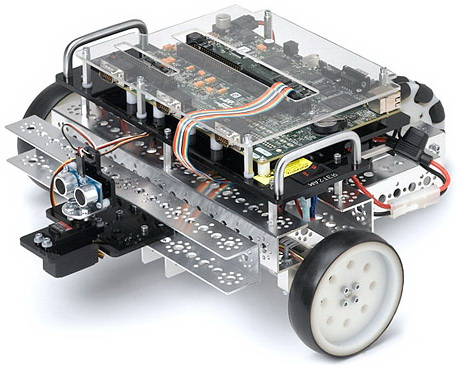
\includegraphics[width=0.75\linewidth]{dani_isometric.jpg}
\centering
\caption{Роботот DaNI}
\label{fig:dani_isometric.jpg}
\end{figure} 

\newpage

\section{DaNI}
National Instruments (NI) LabVIEW комплетот за роботика се состои од DaNI 2.0 (сл.\ref{fig:dani_isometric.jpg}), кој содржи:

\begin{itemize}
	\item Pitsco Education 12 VDC мотори со 152 rpm и 21.6 kg-cm вртежен момент
	\item Оптички квадратурни енкодери со 400 импулси при револуција
	\item PING))) ултразвучен сензор за мерење на растојанја помеѓу 2cm и 3m
	\item PING))) монтажен држач за работен агол од $180 \degree$
	\item Два Pitsco Education TETRIX 10.16cm тркала и едно омни тркало за насочување
	\item sbRIO единица и соодветни кабли за поврзување
\end{itemize}

Хардверот може да биде проучуван, обратно инжениран, и модифициран од студенти. Меѓутоа, главната цел е роботска перцепција и контрола кои се имплементирани во LabVIEW софтвер развиен на одделен сервер (компјутер) и спуштен на роботскиот компјутер.

\begin{figure}[H]
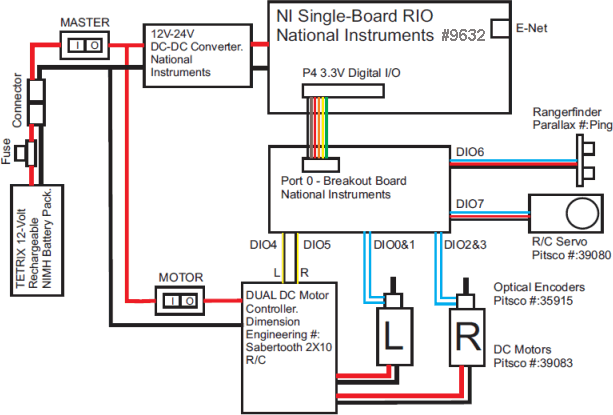
\includegraphics[width=0.75\linewidth]{dani_block_diagram.png}
\centering
\caption{Блок дијаграм на DaNI}
\label{fig:dani_block_diagram.png}
\end{figure}

\subsection{Актуатори}
Од страната на актуатори, DaNI поседува два DC мотори со вградени редуктори, и еден серво мотор. DC моторите се користат за движење на роботот, а серво моторот има улога прецизно да го ротира PING))) ултразвучниот сензор. Подолу се наведени нивните карактеристики.

\subsubsection{DC Мотори}
DC мотор со четкици претставува внатрешно комутиран електричен мотор дизајниран да биде напојуван со извор на еднонасочна струја. Неговата брзина може да се менува со промена на работниот напон или јачината на магнетото поле.
Во DaNI се применети два DC мотори, поточно TETRIX MAX DC мотори(сл.\ref{fig:dc_motor_iso.png}).

\begin{figure}[H]
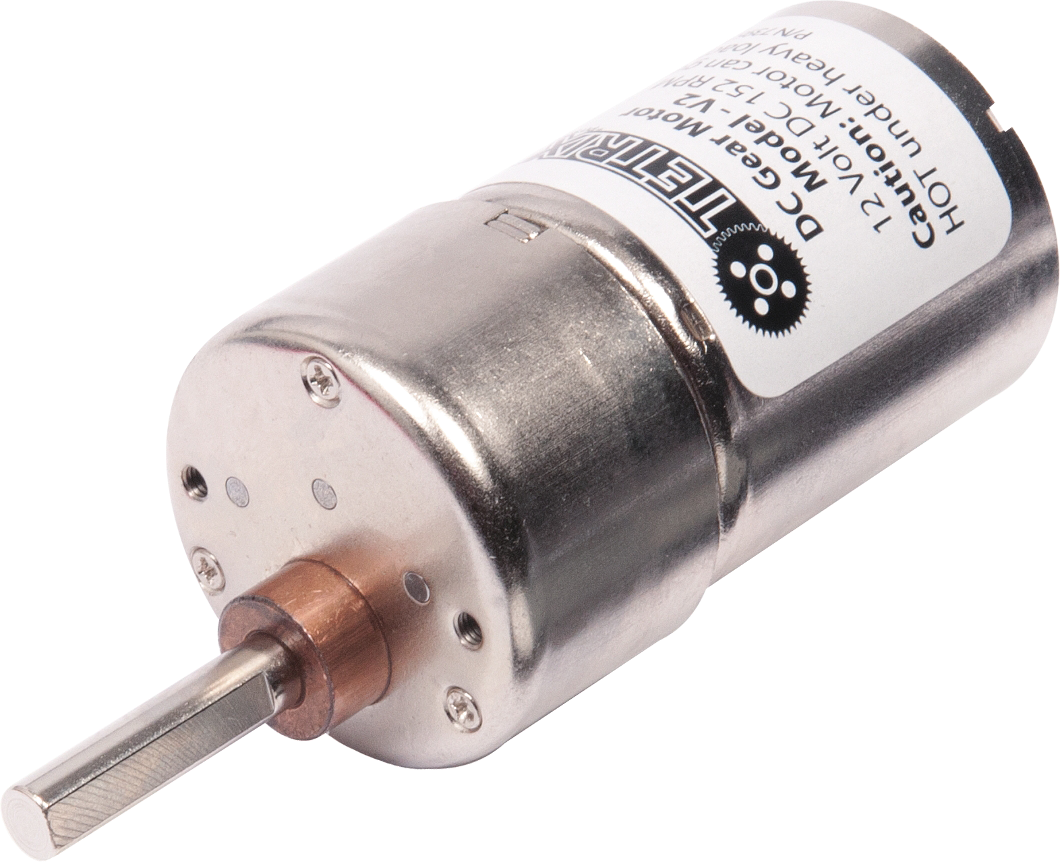
\includegraphics[width=0.35\linewidth]{dc_motor_iso.png}
\centering
\caption{Tetrix Max DC мотор}
\label{fig:dc_motor_iso.png}
\end{figure}

\renewcommand{\theenumii}{\arabic{enumii}}
\renewcommand{\theenumiii}{\arabic{enumiii}}
\begin{enumerate}
	\item При нормални услови на работа:
	\begin{enumerate}
		\item Номинален напон: $ 6-13.8 V $
		\item Температура на околината: $ -10 \pm 60 \degree C $
		\item Насока на ротација: Спротивно од стрелката на часовникот\\Позитивен пол поврзан со црвен „+“\\Негативен пол поврзан со „-“\\Гледајќи кон оската на излезното вратило		
	\end{enumerate}
	\item Услови на испитување:
	\begin{enumerate}
		\item Напон: DC 12 V
		\item Температура на околината: $ 28 \degree C $
		\item Влажност на воздухот: 44 \% RH
		\item Испитуваниот уред е поставен хоризонтално
	\end{enumerate}
	\item Електрични способности(По 30 секунди напојување)
	\begin{enumerate}
		\item Без оптоварување
		\begin{enumerate}
			\item Брзина: 150 $\pm$ 10 RPM
			\item Струја: 0.34А (0.68А max)
		\end{enumerate}
		\item Со оптоварување
		\begin{enumerate}
			\item Вртежен момент: 3.9kg.cm
			\item Струга: 0.91А (1.37А max)
			\item Брзина: 137.5 $\pm$ 10 \% RPM
			\item Вртежен момент на запирање: /
			\item Струја на запирање: /
		\end{enumerate}
	\end{enumerate}
	\item Механички карактеристики
	\begin{enumerate}
		\item Аксијално поместување на вратилото: $\leq$ 0.5mm
	\end{enumerate}
	\item Својства на моторот:
	\begin{enumerate}
		\item Струја без оптоварување: 0.19А
		\item Брзина без оптоварување: 11000 $\pm$ 10 \% RPM
	\end{enumerate}
\end{enumerate}	

Двата DC мотори присутни во конструкцијата се контролирани со помош на Sabertooth Dual 10A Motor Driver. Тој може да напојува два DC мотори со четкици со струја до 10А поединечно, со максимални 15А за кратки временски периоди, со многу тивка операција поради ултрасоничната брзина (32kHz) на контрола на неговите транзистори. Sabertooth исто така претставува првиот синхрон регенеративен мотор драјвер во својата класа. Регенеративната топологија значи дека батериите на уредот се полнат кога на уредот му се наредува да забави или да се врати назад, при што исто така ја зголемува и брзината на реакција. Вклучува внатрешно напојување од 5V кое може да напојува микроконтролер или R/C приемник. 

Наредно се зададени техничката скица(сл.\ref{fig:motor_schematic.png}) на моторот со неговите димензии, како и графикот на карактеристики на моторот за различно оптоварување(сл.\ref{fig:motor_graph.png}). Овој график ги дава целокупните карактеристики, т.е. карактеристиките на моторот заедно со редукторот.

\begin{figure}[H]
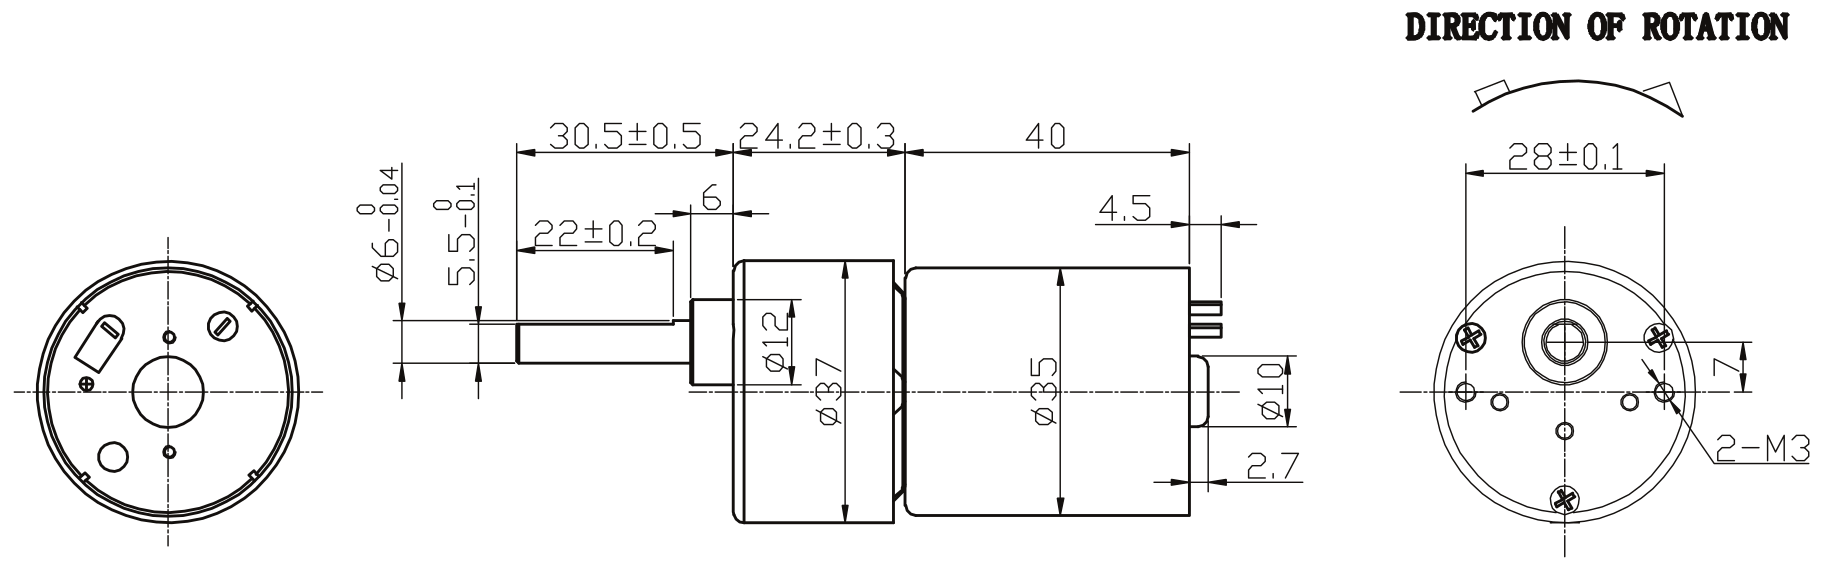
\includegraphics[width=0.75\linewidth]{motor_schematic.png}
\centering
\caption{Техничка скица на DC моторот}
\label{fig:motor_schematic.png}
\end{figure}

\begin{figure}[H]
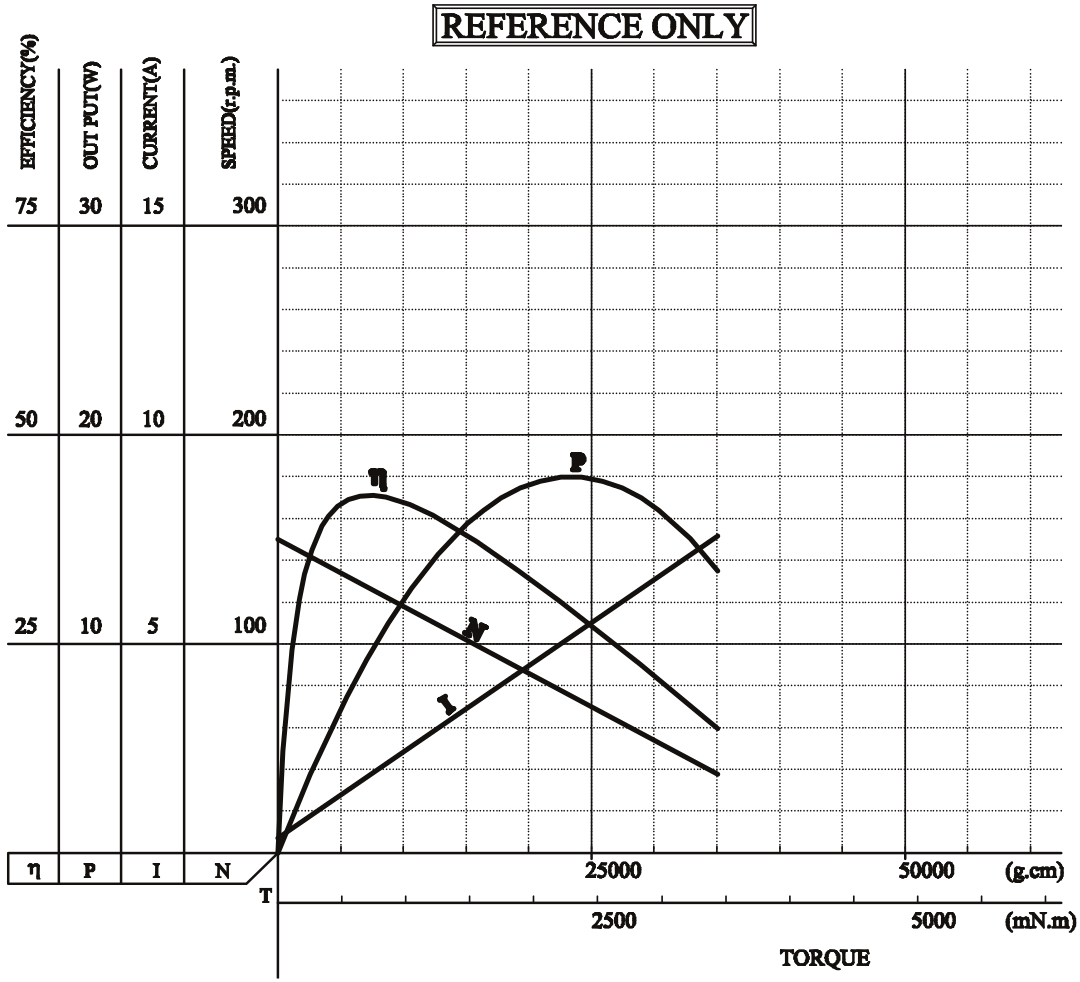
\includegraphics[width=0.75\linewidth]{motor_graph.png}
\centering
\caption{Карактеристични вредности на DC моторот}
\label{fig:motor_graph.png}
\end{figure}

\subsubsection{Серво Мотор}
Серво мотор е ротационен актуатор кој дозволува за прецизна контрола на аголна позиција. Тој се состои од мотор поврзан со сензор за повратни информации за позиција. Исто така има потреба од серво драјвер, кој прима команден сигнал од контролен систем, го засилува сигналот, и пренесува електрична струја до серво моторот со цел да произведе движење пропорционално со командниот сигнал. За оваа цел го користи и сензорот за повратни информации за позиција за да се добие прецизна контрола на ротационата позиција на моторот. Ова е т.н. систем со затворена повратна врска.

Единствена функција на серво моторот во оваа конструкција е ротација на PING))) сензорот, поради што тој не е изложен на значителни оптоварувања.

\begin{table}[h]
\caption{Карактеристики на серво моторот}
\label{tab:title}

\begin{center}
\begin{tabular}{||c|c||}
\hline
Димензии & 39.88 х 19.81 х 37.85mm\\
\hline
Тежина & 45g\\
\hline 
Ранг на напон & 4.8V - 6.0V\\
\hline
Брзина без оптоварување (4.8V) & 0.22sec/60\degree\\
\hline
Брзина без оптоварување (6.0V) & 0.18sec/60\degree\\
\hline
Вртежен момент на запирање (4.8V) & 4.8kg.cm\\ 
\hline
Вртежен момент на запирање (6.0V) & 6.0kg.cm\\
\hline
Максимален ранг на PWM & 553-2425\micro sec\\
\hline
Поминат агол по \micro sec & .102\degree/\micro sec\\
\hline
Максимален пат & 190.5\degree \\
\hline
Амплитуда на импулс & 3-5V \\
\hline
Работна температура & -20\degree C до +60\degree C \\
\hline
Потрошувачка на струја - неактивен (4.8V) & 8mA \\
\hline
Потрошувачка на струја - неактивен (6V) & 8.8mA \\
\hline
Потрошувачка на струја - без оптоварување (4.8V) & 150mA \\
\hline
Потрошувачка на струја - без оптоварување (6V) & 180mA \\
\hline
Можност за континуирана ротација & + \\
\hline
Насока со зголемување на PWM сигнал & Во насока на часовата стрелка \\
\hline
Вид на запченици & Запченици со прави заби \\
\hline
Материјал на запченици & Карбонит \\
\hline
\end{tabular}
\end{center}
\end{table}

\begin{figure}[H]
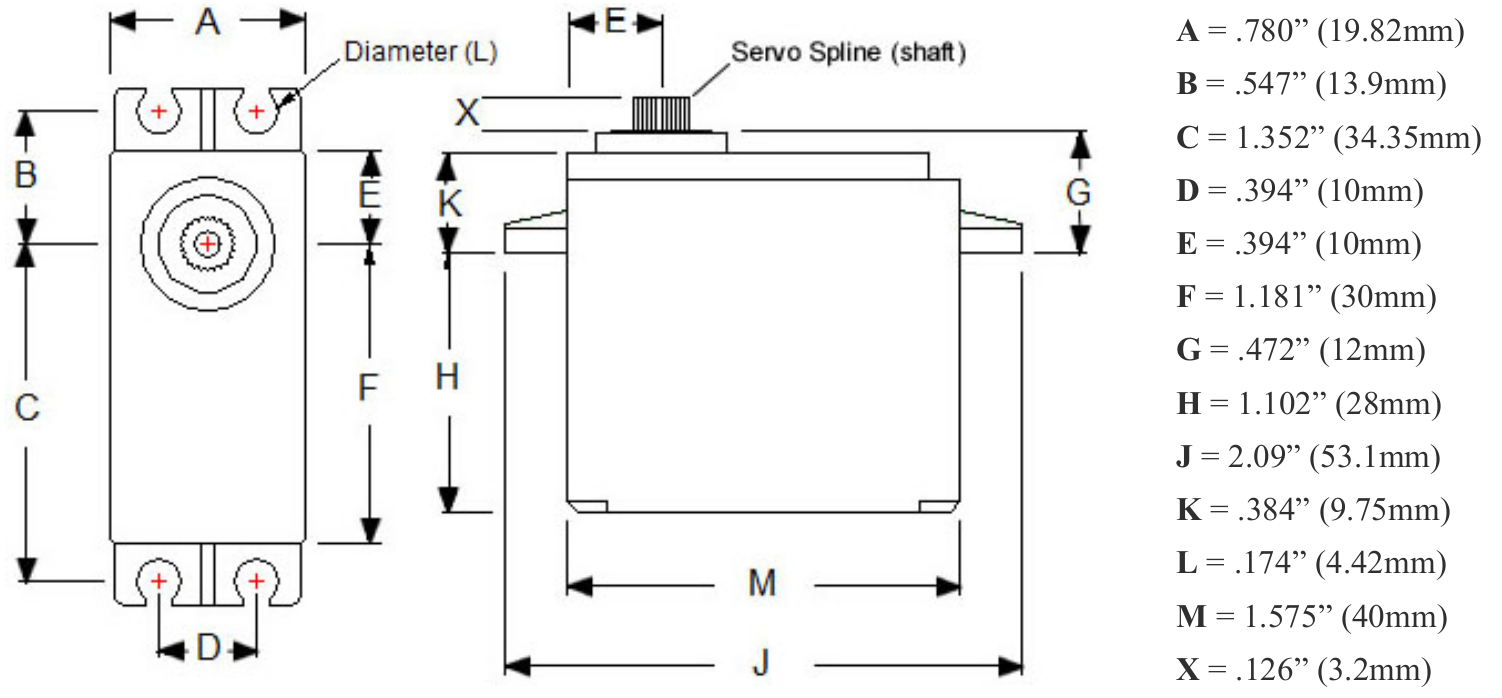
\includegraphics[width=0.75\linewidth]{servo_schematic.png}
\centering
\caption{Димензии на серво моторот}
\label{fig:servo_schematic.png}
\end{figure}

\subsubsection{PWM}
PWM (Pulse Width Modulation) е начин на аналогно управување базиран на употребата на чисто дигитални сигнали. При една претходно одредена фреквенција, имаме една соодветна периода, $T(s)$. Во рамките на една периода, можеме да ја дефинираме врската помеѓу времетраењето на активноста (ОN) и времетраењето на неактивноста (OFF) на еден дигитален излез. Добиениот „аналоген“ излез (ефективниот напон) се пресметува со следната равенка:\\

$$ V_{PWM} = V_{dig} \cdot \frac{T_{ON}}{T_{ON} + T_{OFF}} = V_{dig} \cdot \frac{T_{ON}}{T} $$

На пример, ако имаме работна фреквенција 20kHz, имаме периода $50\mu s$. Нека дигиталниот излез биде 5V (т.е. ON = 5V, OFF = 0V). Ако за $30\mu s$ од секоја периода задаваме ON сигнал, а за останатите $20\mu s$ задаваме OFF сигнал, на излез ќе го добиеме ефективен напон:

$$ V_{PWM} = 5 \cdot \frac{30}{30+20} = 5 \cdot 0.6 = 3V $$

\subsection{Сензори}
Во најширока дефиниција, сензор претставува уред, модул или подсистем чија задача е да препознае настани или промени во својата околина, и да испрати согласна информација кон останатата електроника (најчесто компјутерски процесор).

Во DaNI употребуваме два вида на сензори: енкодер и ултразвучен сензор.

\subsubsection{Енкодер}
Ротационен енкодер, е електромеханички уред кој ја претвора аголната позиција или движење на вратило во аналоген или дигитален сигнал.

Постојат два главни видови: апсолутни и инкрементални (релативни). Излезот од апсолутни енкодери ја изразува моменталната позиција на вратилото, што ги прави аголни трансдусери. Излезот на инкрементални енкодери дава информација за \textit{движењето} на вратилото кое понатаму се процесира во информации како за брзина, растојание и позиција. 

Ротационите енкодери се користат во многу области на апликации кои имаат потреба од прецизна контрола на неограничена ротација на вратило, вклучувајќи индустриски контрола, роботика, фотографски леѓи за специјални примени, компјутерски влезни уреди, и ротациони радарни платформи.

Во нашиот случај, енкодерот е инкрементален квадратурен енкодер(сл.\ref{fig:encoder.png}), што значи дека користи два излеза A и B кои се наоѓаат на 90 \degree фазно поместување еден од друг(сл.\ref{fig:encoder_quadrature.png}).

\begin{table}[h]
\caption{Зголемување на фазата имплицира ротација во насока на стрелките на часовникот}
\label{tab:title}

\begin{center}
\begin{tabular}{||c|c|c||}
\hline
Фаза & A & B \\
\hline \hline
1 & 0 & 0 \\
\hline 
2 & 0 & 1 \\
\hline
3 & 1 & 1 \\
\hline
4 & 1 & 0 \\
\hline
\end{tabular}
\end{center}
\end{table}

\begin{figure}[H]
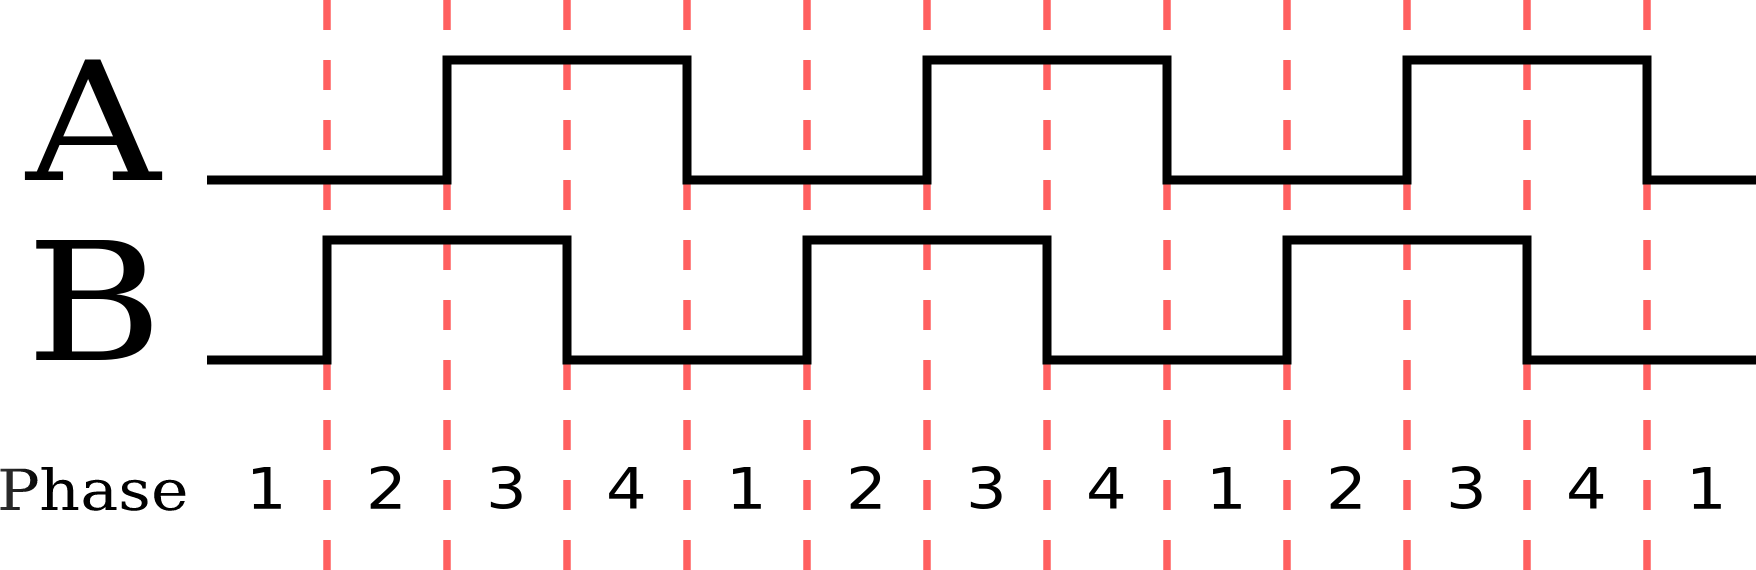
\includegraphics[width=0.5\linewidth]{encoder_quadrature.png}
\centering
\caption{Два квадратни бранови во квадратура (ротација во насока на стрелките на часовникот)}
\label{fig:encoder_quadrature.png}
\end{figure}

Исто така дискот има 400 отвори, односно енкодерот има резолуција од 0.9\degree.

\begin{figure}[H]
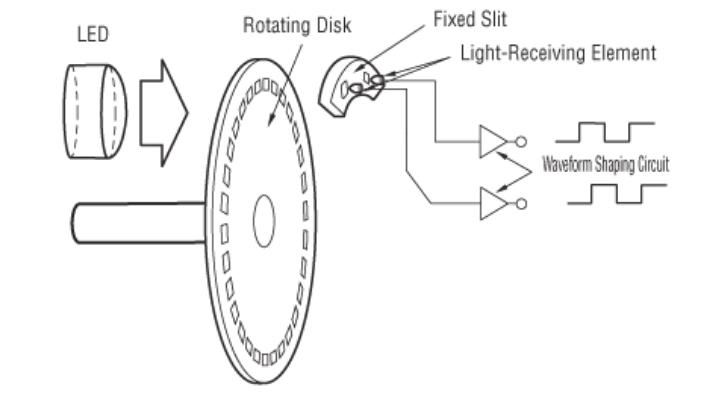
\includegraphics[width=0.5\linewidth]{encoder.png}
\centering
\caption{Шема на оптички енкодер}
\label{fig:encoder.png}
\end{figure}

\subsubsection{Ултразвучен Сензор}
Ултразвучниот сензор PING))) од Паралакс(сл.\ref{fig:ping_dims.png}) е способен да извршува прецизни мерења на растојанија од 2cm до 3m. Лесно се приклучува на микроконтролери како BASIC Stamp, Propeller chip, или Arduino, користејќи само еден I/O пин. Се напојува со 5V и 30mA.

PING))) сензорот работи со пренесување на ултрасончен (високо над осетливиот ранг на човекот) збир (burst) на бранови, и произведува излезен пулс кој соодветствува на времето потребно за ехото на брановите да се врати до сензорот. Со мерење на ширината на излезниот пулс, лесно може да се пресмета растојанието до објектот.

\begin{figure}[H]
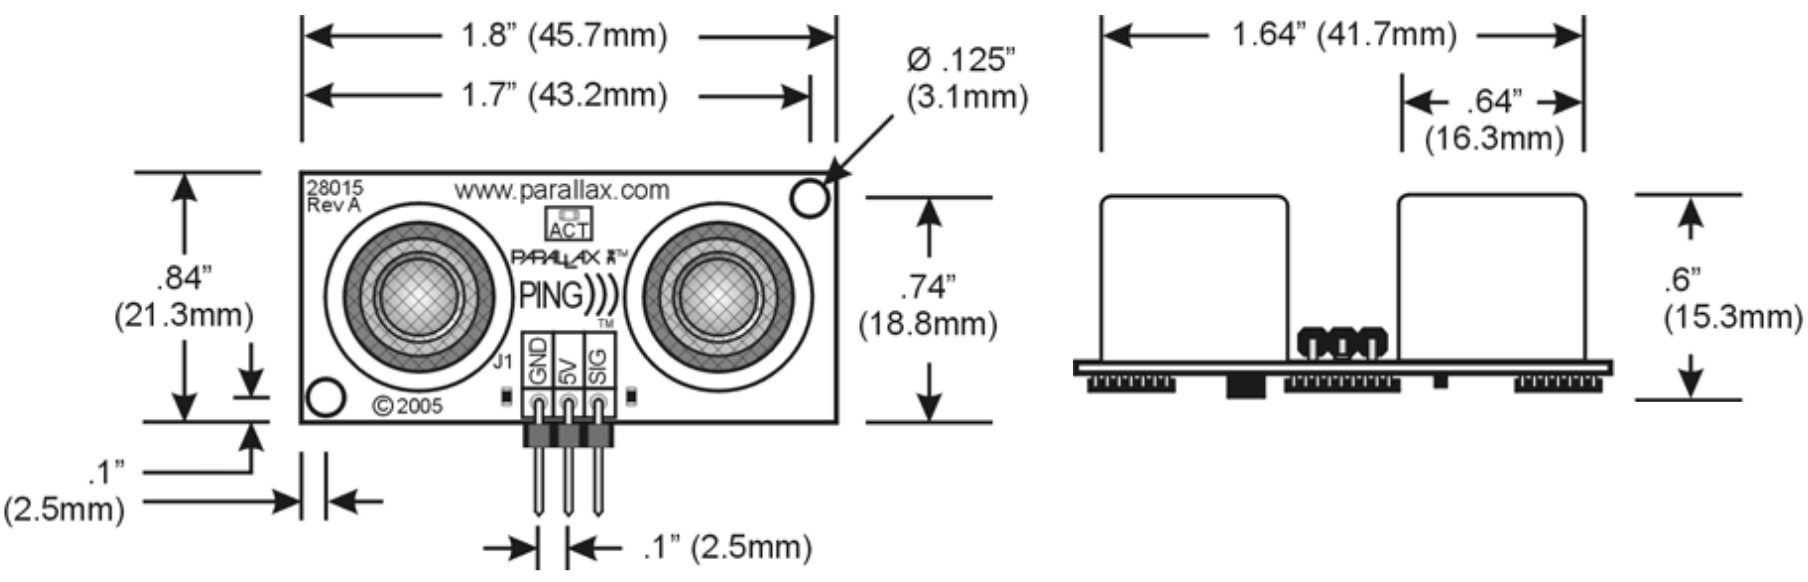
\includegraphics[width=0.75\linewidth]{ping_dims.png}
\centering
\caption{Димензии на PING))) сензорот}
\label{fig:ping_dims.png}
\end{figure}

\begin{figure}[H]
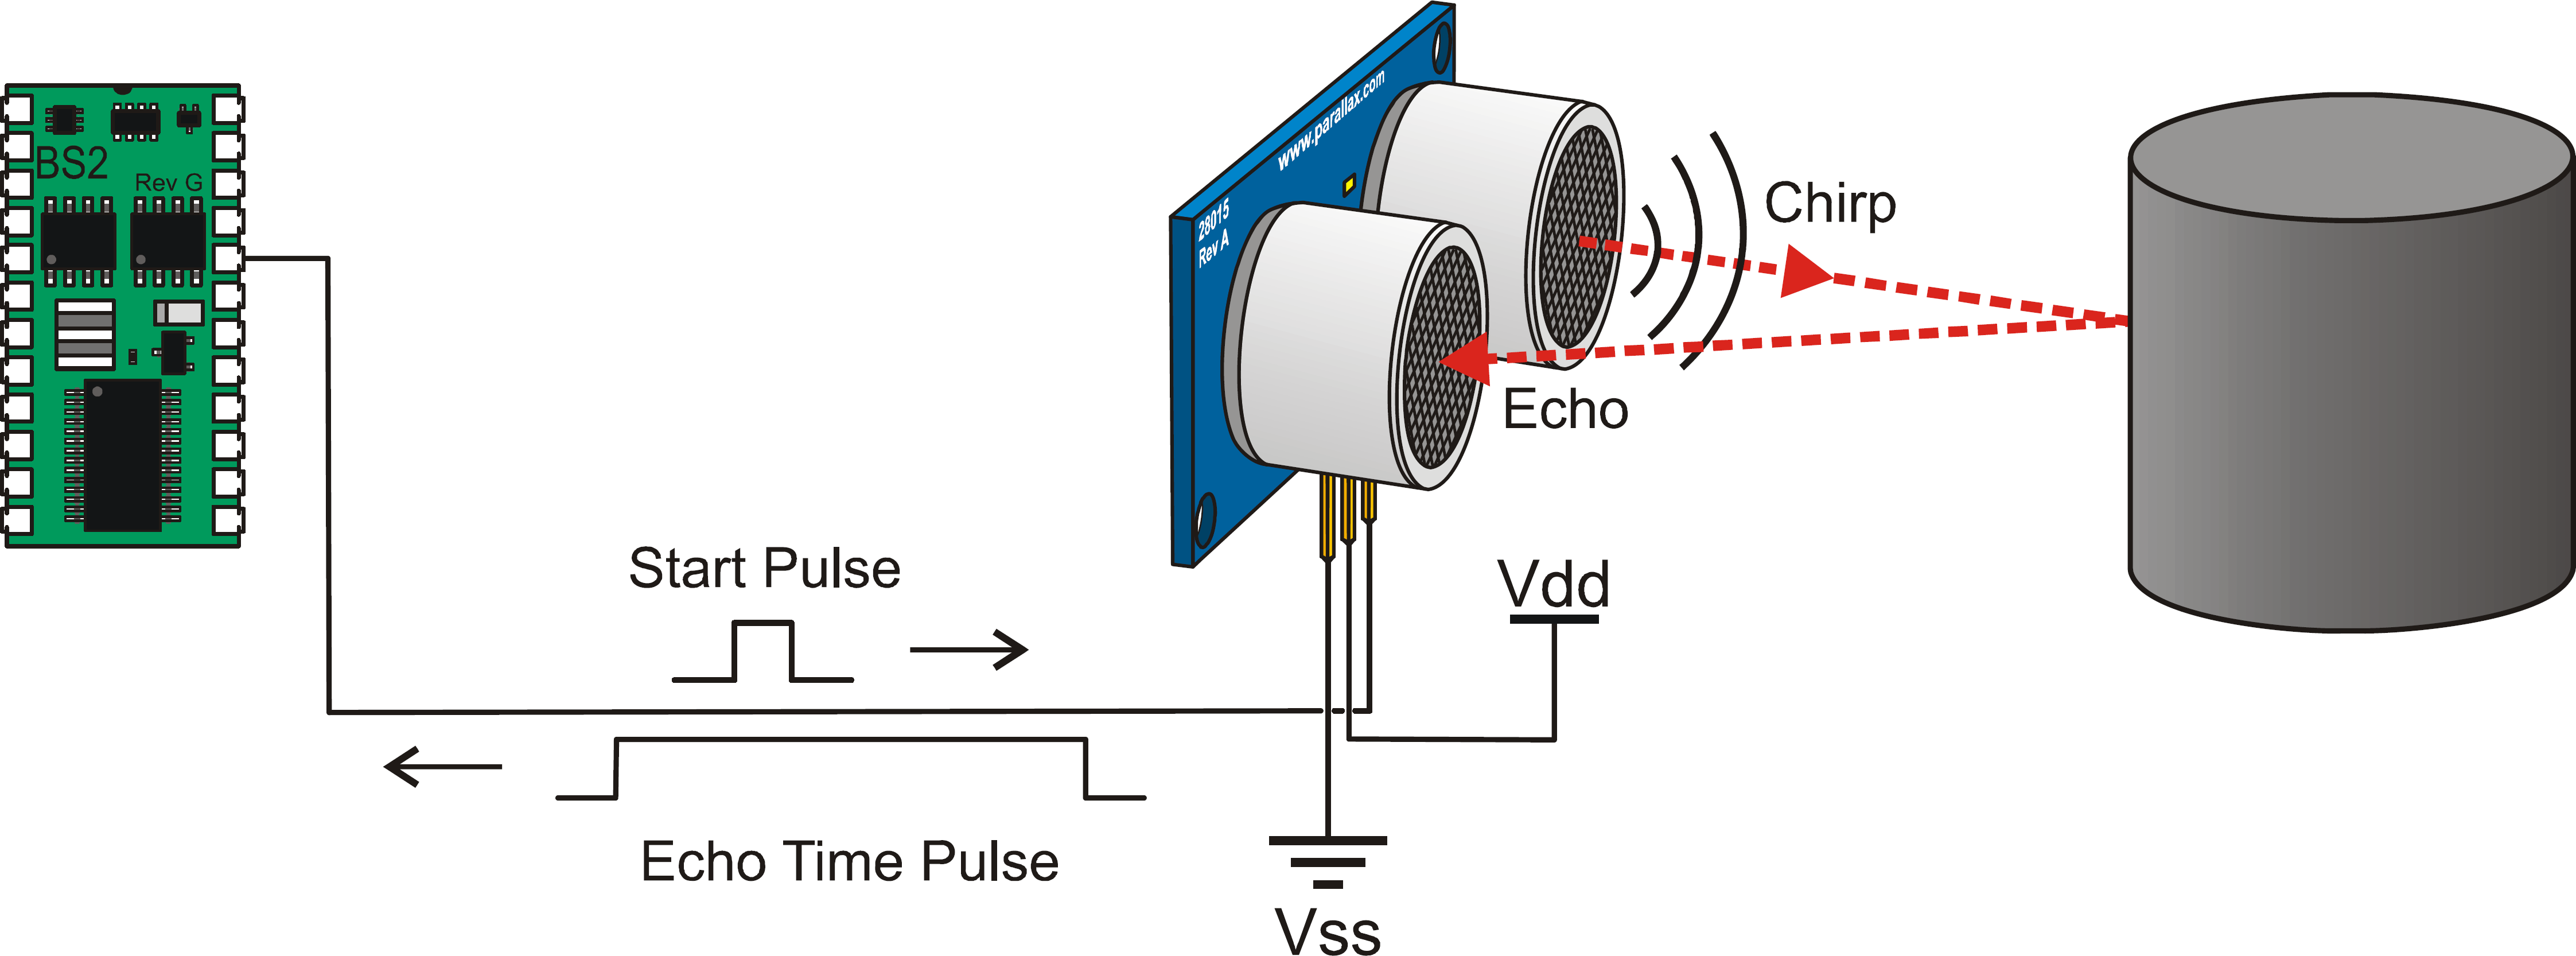
\includegraphics[width=0.75\linewidth]{ping.png}
\centering
\caption{Шема и принцип на дејство на ултразвучен сензор}
\label{fig:ping.png}
\end{figure}

\paragraph{Протокол на комуникација\\}
PING))) сензорот детектира предмети со емитирање на краток ултрасоничен збир (burst) на бранови, и потоа со „слушање“ за ехото. Под контрола на главен микроконтролер (пулс на активација), сензорот емитира краток 40kHz сигнал. Овој сигнал патува низ воздухот, се судира со објект и се одбива назад кон сензорот. Истовремено сензорот испраќа излезен пулс на микроконтролерот кој ќе се прекине штом се детектира ехото, кој всушност ни го дава растојанието до предметот(сл.\ref{fig:ping.png}).

\begin{figure}[H]
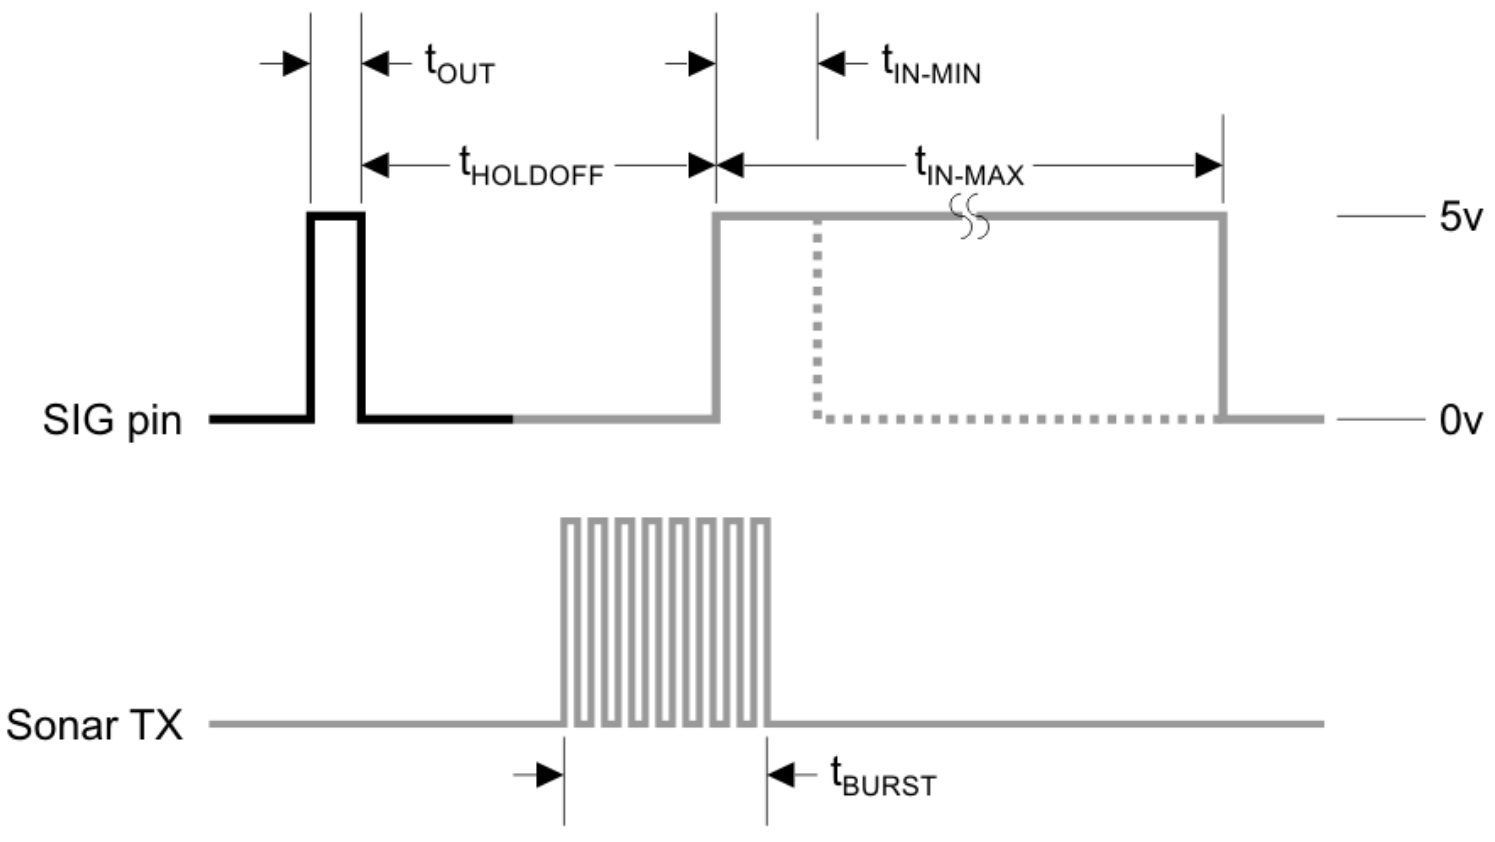
\includegraphics[width=0.75\linewidth]{ping_sig.png}
\centering
\caption{Изглед на сигналот}
\label{fig:ping_sig.png}
\end{figure}

\begin{table}[H]
\caption{Карактеристики на сигналот}
\label{tab:title}

\begin{center}
\begin{tabular}{||c|l|l|l|l||}
\hline
Темна линија & Главен Уред & Влезен пулс на активација & $ t_{OUT} $ & $2\mu s$ (min), $5\mu s типично$ \\ \hline
\multirow{5}{*}{Светла линија} & PING))) Сензор & Задржување на ехо & $ t_{HOLDOFF} $ & $750\mu s$ \\
 & & Фреквенција на сигналот (burst) & $ t_{BURST} $ & $ 200\mu s $ @ $ 40kHz $ \\
 & & Ехо повратен сигнал минимум & $ t_{IN-MIN} $ & $ 115\mu s $ \\
 & & Ехо повратен сигнал максимум & $ t_{IN-MAX} $ & $ 18.5\mu s $ \\
 & & Пауза пред следно мерење & & $ 200\mu s $ \\
\hline
\end{tabular}
\end{center}
\end{table}

\paragraph{Позиционирање на објектот\\}
PING))) сензорот не може прецизно да измери растојание до објект кој што:

\renewcommand{\theenumi}{\alph{enumi}}
\begin{enumerate}
	\item се наоѓа подалеку од 3m
	\item има мал агол на рефлектирачката површина со што сигналот нема да биде одбиен назад кон сензорот
	\item е премногу малечок за да рефлектира доволно звук назад кон сензорот.
\end{enumerate}

Исто така, доколку PING))) сензорот е поставен на ниска позиција на уредот, има можност да детектира звук кој се одбива од подот.

\begin{figure}[H]
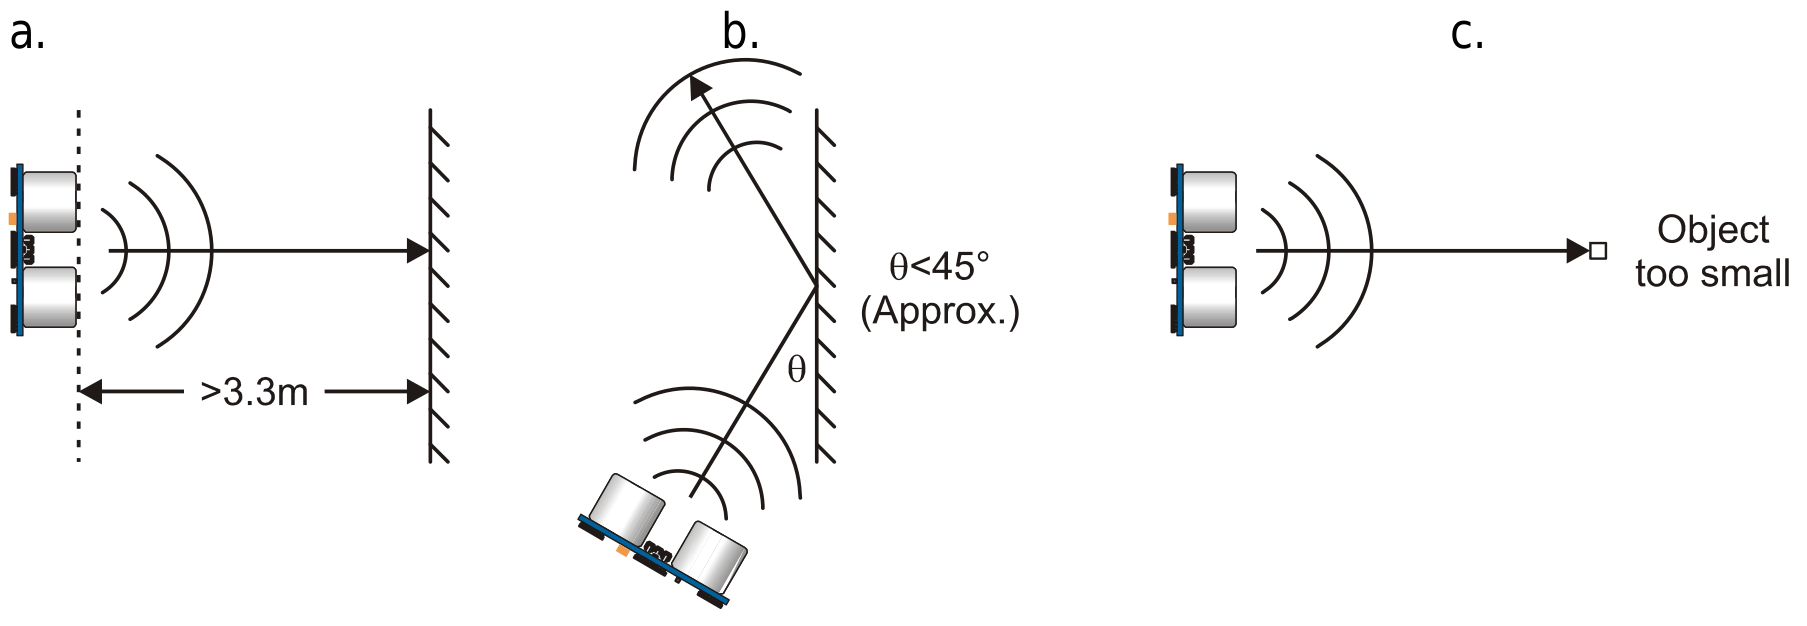
\includegraphics[width=0.75\linewidth]{ping_obj.png}
\centering
\caption{Позиционирање на објектот}
\label{fig:ping_obj.png}
\end{figure}
\newpage

\section{NI sbRIO 9632}
\begin{figure}[h]
\centering
\includegraphics[width=0.75\linewidth]{sb_rio_1.png}
\caption{sbRIO со обележани компоненти}
\label{fig:sb_rio_1.png}
\end{figure}

sbRIO (single-board Reconfigurable Input/Output) управувачките единици од National Instruments претставуваат компјутер монитран на една плочка (single board) наменета за случаи каде што е потребно решение со управување во реално време (Real Time). Оперативен систем кој работи во реално време (RTOS: Real Time Operating System) е изработен со особената цел да извршува функции кои барат големо ниво на временска прецизност и висок степен на надежност. За некој систем да се смета за RTOS, тој мора да има познато максимално време на извршување за секоја од неговите клучни операции. Системите кои можат сигурно да обезбедат максимален временски одѕив се вели дека работаат во потполно реално време, додека системите кои можат само понекогаш да обезбедат максимален временски одѕив се вели дека работаат во делумно реално време.
 
Потребната брзина се постигнува со истовремето користење на FPGA чип и една обична линеарна процесорска единица. 

sbRIO поседува 110 дигитални влезови/излези, 100 од кои се оспособени за PWM (Pulse Width Modulation), а 10 од кои се наменети за ниско-фреквентна намена. sbRIO поседува и 32 аналогни влезови, и 4 аналогни излези со ранг на излез од $ \pm 10\ V$ со $0.1\%$ грешка при типична употреба на $25\degree C \pm5\degree C$.

sbRIO содржи и 3 сериски „С“ портови за поврзувањето на надворешни модули од NI за проширување на можностите на sbRIO да опфатат и актуација и аквизиција на податоци.

\subsection{FPGA}
FPGA, или „Field Programmable Gate Array“, претставува репрограмибилно интегрално коло кој поседува голем број на програмибилни логични порти. Кај обичните микроконтролери, логиката за управување се пишува и компајлира од некои програмски јазик како C, BASIC или некој графички јазик како G (LabVIEW). Во текот на овој процес се сублимираат во процесорски наредби како ADD и MOV. Низата на можните наредби е единствена за секој микропроцесор. Кај FPGA колата, програмата не се сублимира на наредби, туку самата внатрешна архитектура на колото се подредува со електромагнетни полиња. Како резултат, се добива конфигурација на логични порти која ќе ја извршува задачата опишана во првобитната програма. Бидејќи FPGA нудат хардверско решение, нивното работење е често многу пати побрзо од работењето на обичните микроконтролери, но се подраги.

\begin{figure}[h]
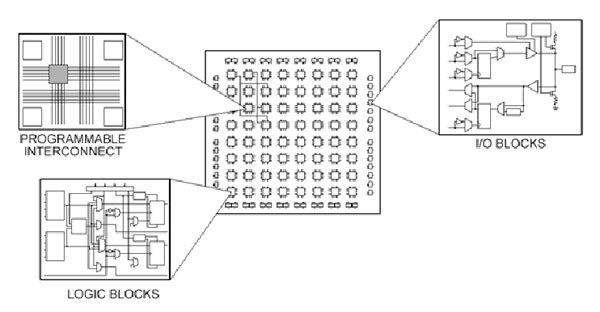
\includegraphics[width=0.75\linewidth]{fpga_diagram.jpg}
\centering
\caption{Приказ на често сретнати термини кај FPGA кола}
\label{fig:fpga_diagram_jpg}
\end{figure}

FPGA колото што се наоѓа во sbRIO-то е моделот Xilinx Spartan 6, кој поседува 6 милиони репрограмибилни логични порти.

\subsection{Споредба со Ардуино Уно}
Ардуино претставува често применето open-source решение за управувачки задачи и во индустрија и на аматерскиот терен. Ардуино плочи често содржат микроконтролер, аналогни-дигитални и дигитални-аналогни претворувачи, и осцилаторски кристал. Додека sbRIO плочите се програмираат во LabVIEW, Ардуино плочите се програмираат во сопствениот „Ардуино“ јазик, која е проширена и поедноставена варијанта на C++ јазикот. Ардуина се популарни помеѓу хобисти, студенти, и за прототипување. Најпопуларната варијанта на Ардуино плочите е Ардуино Уно, која е споредена со sbRIO-то подолу:  

\begin{table}[h]
\caption{Споредба помеѓу Arduino Uno и sbRIO}
\label{tab:title}

\begin{center}
\begin{tabular}{||c|c|c||}
\hline
  & Arduino Uno & NI sbRIO 9632 \\ [0.75ex]
\hline \hline
Напојување & 7 - 12 V DC & 19 - 30 V DC \\
\hline 
Дигитален I/O & 14 влезови/излези & 110 влезови/излези \\
\hline
Брзина & 16MHz & 400MHz \\
\hline
Аналогни влезови & 6 влезови & 32 single-ended влезови \\
\hline
Аналогни излези & 6 дигитални пинови способни за PWM & 4 16-bit излези, 100 PWM пинови \\
\hline
Меморија & 2kB RAM, 32kB неволатилна & 128MB RAM, 256MB неволатилна \\ 
\hline
Цена & €15 & €1560 \\ [0.5ex]
\hline
\end{tabular}
\end{center}
\end{table}
\newpage

\section{LabVIEW}
LabVIEW (Laboratory Virtual Instrument Engineering Workbench) е софтверски пакет наменет за програмирањето на виртуелни уреди (инструменти) за мониторинг и управување на физички уреди. Инструментите што се програмираат во LabVIEW можат да се компајлираат и да се издават како комплетно независни програми кои можат да се монтираат како главен управувен софтвер на мехатроничките уреди и машини. LabVIEW инструментите се програмираат користејќи го нивниот сопствен графички програмски јазик, „G“. Да се спомени дека јазикот G и G-Code немат никаква поврзаност меѓу себе.

Основниот пакет на LabVIEW поседува многу од стандардните можности што се очекуваат од било кој програмерски јазик, како што се логички/булови операции, математички операции, и пристап до алатки за визуелизација на податоци. 

LabVIEW може да се прошири (и во некои случаи мора да се прошири) со додатни пакети. На пример, овие пакети можат да содржат готови под-инструменти (sub-VIs) за обработка на сигнали (Signal Processing ), или да овозможуваат соработка помеѓу LabVIEW и некои други технологии (FPGA module). Од овие пакети ние ги употребуваме Real Time, FPGA, и Robotics пакетите. Првите два пакети ни го оспособуваат LabVIEW да програмира FPGA чипови и да управува во реално време, додека Robotics пакетот содржи во себе голем број на готови инструменти за обична и инверзна кинематика, отчитување од сензори, и праќање наредби на моторите. 

Robotics пакетот исто поседува едно подмножество на инструменти наменети само за DaNI 2.0, и со тие го управувавме DaNI роботот.

\subsection{Robotics Модул: Starter Kit 2.0}
Во Robotics модулот на LabVIEW, од интерес ни се готовите VIs за Starter Kit 2.0, кои содржат во нив потпрограми за иницијализација и деиницијализација на роботот, отчитување од сензорите, и задавање на брзина на ротација на моторите. Тука ќе се набројат и објаснат овие блокови.

\paragraph{Иницијализација:\\}

\begin{figure}[h]
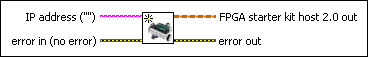
\includegraphics[width=0.45\linewidth]{init.png} 
\raggedright
\caption{VI за иницијализација}
\label{fig:init.png}
\end{figure}

Првиот блок служи за иницијализацита на роботот. Како влез се доведува IP адресата на DaNI роботот, и според зададената адреса започнува комуникацијата со DaNI. При иницијализација на DaNI се создава „објект“ кој го претставува роботот. Програмерскиот термин „објект“ дефинира конгломерат на податоци и функции коj го опишува некој апстрактен предмет. Овие предмети се често неопипливи, но во случаи како нашиот, овој „објект“ е еден кибернетски претставнички меѓуслој кој ни овозможува комуникација со физичкиот систем во прашање. Како излез на оваа функција го добиваме објектот на DaNI, што ни претставува предуслов за употребата на било која од другите фунцкии. Error-in и error-out портите на VI-то се за заштита при некоја грешка во системот. Ако грешката е 1 (има грешка), целата функцијата на иницијализација се заменува со куса врска, и нема излезен објект. \\

\paragraph{Деиницијализација:\\}
\begin{figure}[h]
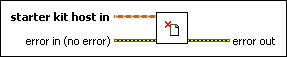
\includegraphics[width = 0.45\linewidth]{deinit.png}
\raggedright
\caption{VI за деиницијализација}
\label{fig:deinit.png}
\end{figure}

Овој блок се става на крај на програма за да се избрише објектот создаден од иницијализацијата, и да се направи соодветен излез. Без оваа крајна фунцкија, грешки се појавуваат при рестартирање на роботот и промени на програмата. 
\\

\paragraph{Управување на моторите:\\}
\begin{figure}[h]
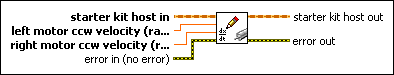
\includegraphics[width=0.45\linewidth]{write_dc.png}
\raggedright
\caption{VI за дефинирање на брзина}
\label{fig:write_dc.png}
\end{figure}

Овој блок е должен за управувањето на брзината на двата DC мотори на DaNI. За функционирањето на блокот потребен е самиот објект на DaNI, како и две вредности за врзините на моторите во \textit{rad/s}. За движење во било која насока, важно е да се опомени дека брзините на моторите морат да бидат со обратен предзнак порадни ниваната обратна поставеност. Моторите имаат максимална брзина на 15.7 \textit{rad/s}.

\paragraph{Отчитување од енкодерите:\\}
\begin{figure}[h]
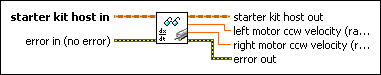
\includegraphics[width=0.45\linewidth]{read_dc.png}
\raggedright
\caption{VI за отчитување од енкодерите}
\label{fig:read_dc.png}
\end{figure}

Со овој блок се отчитуваат моменталните вредности од енкодерите на двата мотори на DaNI. Излезните вредности се во \textit{rad/s} и имаат \textit{float} формат, и заради тоа можат директно да се прикажат на \textit{display}, во \textit{chart} да се претставаат, или да се вклучат во други пресметки или контролери.

\paragraph{Отчитување од ултразвучниот сензор:\\}
\begin{figure}[H]
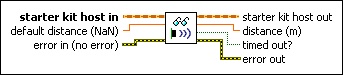
\includegraphics[width=0.45\linewidth]{read_ping.png}
\raggedright
\caption{VI за отчитување од ултразвучниот сензор}
\label{fig:read_ping.png}
\end{figure}

Овој блок служи за отчитување на информацијата дадена од ултразвучниот сензор, монтиран врз серво мотор на предниот дел од DaNI. Отчитаните вредности се исто во формат \textit{float} и се во мерна единица метри.

\paragraph{Насочување на ултразвучниот сензор:\\}
\begin{figure}[H]
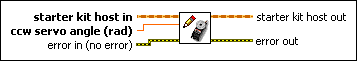
\includegraphics[width=0.45\linewidth]{write_servo.png}
\caption{VI за насочување на ултразвучниот сензор}
\label{fig:write_servo.png}
\raggedright
\end{figure}
Со овој блок се управува серво моторот на DaNI, односно се одредува поставеноста на ултразвучниот сензор. Блокот како влезови ги прима објектот на DaNI и посаканиот агол во радијани. Право пред роботот се смета за 0, позитивни вредности го вртат сензорот на лево, додека негативни вредности го вртат сензорот на десно. Доменот на сензорот е $ \pm \frac{\pi}{2}$, или $\pm 90 \degree$.

\newpage
\section{Управување со повратна врска}
\subsection{ПИД контролери}
\subsubsection{Линеарни закони за управување}
Линеарните закони за управување претставуваат едни од најстарите и најраспространетите управувачки стратегии. Причината за тоа е фактот што со примена на оваа стратегија можат да се решат дури 90\% од сите управувачки задачи. Конечно, овие техники на подесување на параметри на овие закони за управување се детално разработени и многу едноставни за практична примена.\\
Линеарните закони за управување се остваруваат со три дејствија:
\begin{itemize}
	\item Пропорционално (P)
	\item Интегрално (I)
	\item Диференцијално (D)
\end{itemize}

Па оттука уредот со кој ова управување се реализира се нарекува пропорционално-интегрално-диференцијален регулатор или накратко PID. Законите за управување може да се претстават како:

$$ u(t) = K_{p}e(t)+\frac{K_{p}}{T_{i}}\int_{0}^{t}{e(\tau)d\tau} + K_{p}T_{d}\frac{de(t)}{dt} $$

Така што преносната функција на PID e:

$$ G(s) = K_{p}(1+\frac{1}{T_{iS}}+T_{d}S) $$

Перформансот на системот управуван од PID контролерот зависи од изборот на параметри кои го дефинираат интензитетот на секое од трите дејства. Без разлика од типот на регулаторот или неговата реализација, основните барања за регулација на системот се стабилноста, точноста и брзината на одзивот. Поради тоа е важно да се разгледа ефектот на секое од овие дејства на системот поединечно. 

\begin{figure}[H]
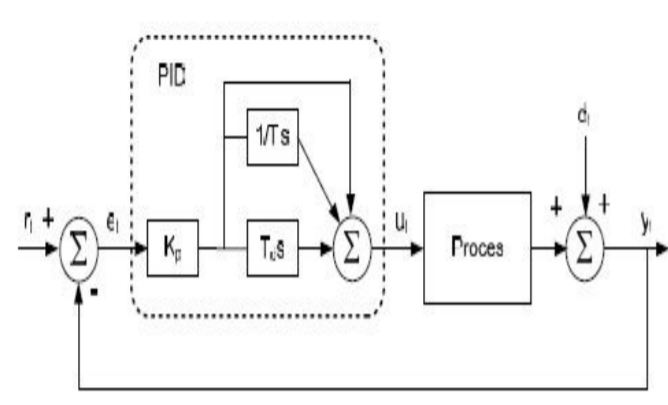
\includegraphics[width=0.5\linewidth]{li_za_up.png}
\centering
\caption{Линеарни закони за управување}
\label{fig:li_za_up.png}
\end{figure}

\subsubsection{Пропорционално дејство}
Пропорционалното дејство ја одредува големината на статичката грешка во системот. Со негово зголемување, грешката се намалува. Меѓутоа во зависност од типот на системот кој се управува, зголемувањето на Кр може да доведе до нестабилен систем (сл.\ref{fig:el_2.png}). Во секој случај, бидејќи постоењето на статична грешка зависи од редот на астатизмот на повратната преносна функција, пропорционалниот коефициент на дејство не може да го промени типот на статичка грешка, туку само нејзината големина. Потребно е да се внимава на фактот дека кај пропорционалното управување нулта статичка грешка имплицира и нулто управување, а тоа значи и прекин на било какви активности во процесот.
Кај некои системи можно е и посакуваниот перформанс да се оствари исклучиво со помош на ова дејство така што управувањето се реализира исклучиво со пропорционален регулатор.
Пропорционалниот регулатор е наједноставен тип на регулатор кој што се опишува со равенката $ u(t) = K_{p}e(t) $ каде што $ K_{p} $ претставува фактор на пропорционално дејство или појачување на регулаторот а $ e(t) $ e грешка на сигнал. Секој пропорционален регулатор се одликува со својата пропорционалност која се дефинира како потребна процентуална промена на влезот, така што излезот би се променил за 100\%. Пропорционалнотото подрачје може да се дефинира како реципрочна вредност од факторот на појачување иразена во проценти. Со појачување на факторот $ K_{p} $, односно намалување на пропорционалното подрачје, константноо се отстапува управувањето на променливата од нејзината зададена вредност, т.е таа се намалува. Во исто време се зголемува брзината на реагирање. На слика \ref{fig:el_3.png} е прикажано дејствувањето на Р регулаторот ако на неговиот влез се додаде грешка на сигнал во облик на отскочна функција.

\begin{figure}[H]
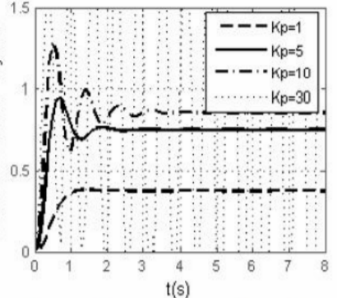
\includegraphics[width=0.3\linewidth]{el_2.png}
\centering
\caption{Отскочен одзив при промена на пропорционален коефициент}
\label{fig:el_2.png}
\end{figure}

\begin{figure}[H]
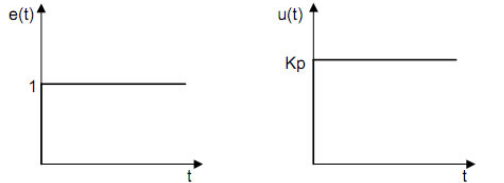
\includegraphics[width=0.3\linewidth]{el_3.png}
\centering
\caption{Дејствување на P регулатор}
\label{fig:el_3.png}
\end{figure}

\subsubsection{Интегрално дејство}
Интегралното дејство има особина да при нулти влез во интеграторот, на излез да добие константен сигнал. Од тука, интегралното дејство во одредена смисла го исправи недостатокот на пропорционалното дејство, односно се додека постои грешка, колку и да е таа мала излезот од интеграторот ќе се менува, а со тоа и самиот сигнал на управување. I регулаторот се опишува со равенката $ u(t) = K_{i}\int_{0}^{t}{e(t)dt} $ која пропорционално ја врзува грешката $ e(t) $ со брзината на управувачка променлива $ u(t) $. Реципрочната вредност на појaчувањето $K_{i}$ е константата $T_{i}$ и претставува време на интегралното дејство $K{i}=\frac{1}{T_{i}}$. Главен недостаток на овој тип на регулатор е дестабилизацијата на системот проследено со за него својственото каснење. На слика \ref{fig:el_5.png} е прикажано делувањето на интегралниот регулатор, ако за влез се донесе грешка $e(t)$ во облик на единечна отскочна функција.

Промената на побуда на системот ќе резултира во промена на одзивот на сигналот кој ќе се (при услов да е системот правилно проектиран), ќе се приближува до зададен референтен сигнал.

Потребно е да се истакне дека оваа особина на интеграторот е многу корисна кај системи чии извршни органи имаат мртва зона која престанува да реагира на побуди.

Грешката акумулирана низ интеграторот ќе го одржува нивото на побуда на извршниот орган надвор од мртвата зона се додека одзивот на системот не се изедначи со референцата.

\begin{figure}[H]
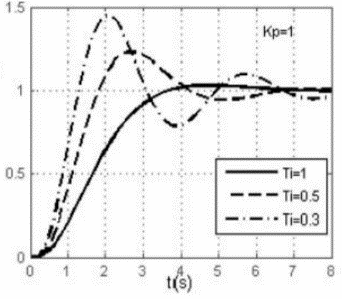
\includegraphics[width=0.3\linewidth]{el_4.png}
\centering
\caption{Отскочен одзив при промена на интегрален коефициент}
\label{fig:el_4.png}
\end{figure}

\begin{figure}[H]
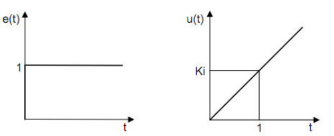
\includegraphics[width=0.3\linewidth]{el_5.png}
\centering
\caption{Дејствување на И регулатор}
\label{fig:el_5.png}
\end{figure}

Примената на интегралното дејство доведува до успорување на одзивот и во однос на пропорционалното дејство. Причина за таквото однесување е тоа што при нагла промена на сигналот, грешката на излезот на интегрсторот расте многу поспоро од излеот на појачување кај пропорционалното управување. Меѓутоа по некое извесно време, излезот на интеграторот, кој всушност го акумулира, односно собира сите претходни вредности на грешката, значајно се зголемува со што се добива осцилаторно однесување на одзивот.

За да се избегне успорувањето на одзивот при промена на сигнал, интегралното дејство никогаш не се користи само, туку исклучиво во комбинација со пропорционалното дејство како PI регулатор. Со подесување на P и I дејството на системот може да постигне извесно подобрување на одзивот на системот, при што се прави ‘компромис‘ помеѓу брзината на одзивот и големината на прескокот. Управување со PI регулаторот е опишано со следната равенка $u(t) = K_{p}e(t)+K_{i}\int_{0}^{t}{e(t)dt}$. Ако на влезот на PI регулаторот се појави сигнал во облик на отскочна функција, пропорционалниот член ќе постави излез $u(t)$ на вредност $K_{p}$, а под дејство на интегралниот член, $u(t)$ ќе продолжи да расте и во моментот $T_{i}$ вредноста на излезот ќе биде еднаква на $2K_{p} = 2(K_{i}T_{i})$. Со други зборови, времето потребно за интеграција е времето потребно а излезот под дејство на интегралниот член, да ја промени вредноста добиена со пропорционалниот член (слика \ref{fig:el_6.png} и слика \ref{fig:el_7.png})

При посакувана брзина на одзивот, прескокот може да се намали само со воведување на диференцијално дејство.

\begin{figure}[H]
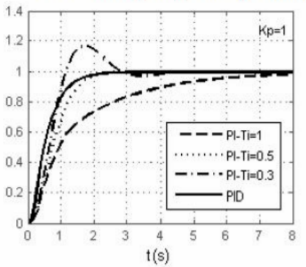
\includegraphics[width=0.3\linewidth]{el_6.png}
\centering
\caption{Отскочен одзив при ПИ и ПИД регулатори}
\label{fig:el_6.png}
\end{figure}

\begin{figure}[H]
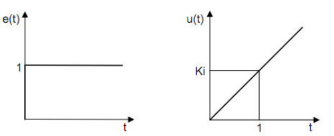
\includegraphics[width=0.3\linewidth]{el_5.png}
\centering
\caption{Дејствување на ПИ регулатор}
\label{fig:el_7.png}
\end{figure}

Диференцијалниот регулатор се опишува со равенката $u(t) = K_d\frac{de(t)}{dt}$. 
Самостојното постоење на диференцијалниот регулатор нема многу смисла, бидејќи кога сигналот на грешка е константен, изводот на овој сигнал е нула. Диференцијалниот регулатор реагира само на брзи промени, додека спорите и долготрајни промени не би предизвикале никакво дејство на овој регулатор. Диференцијлното дејство води сметка за промена на брзината на грешката на сигналот. Доколку не сакаме да имаме прескок во одзивот, неопходно е системот да ‘кочи‘, односно да се успорува промената на одзивот кога грешката на сигналот ќе се намали. 

Очигледно е дека изводот на грешката впрочем ја дава потребната информација за брзинста и смерот на промена на грешка на сигналот.Имајќи во предвид да секој процес има одредена динамика, потребно е некое време да пројде пред да се приметат ефектите од промена на сигналот. Диференцијалното дејство може да се интегрира и како еден вид на предвидувач на грешка на сигнал (слика \ref{fig:el_8.png}). Во пракса диференцијалното дејство покажува значајни недостатоци кои потекнуваат од мерниот шум на излезот.

Често користен, а воедно и применет во нашиот проект е пропорционално-диференцијалниот генератор односно PD. PD регулаторот опишан со следната равенка: $u(t)=K_{p}e(t)+K_{d}\frac{de(t)}{dt}$. Бидејќи станува збор за диференцијално дејство, ќе набљудуваме пореметување $e(t)$ во облик на нагибна функција. Ако на влезот на PD регулаторот доведеме нагибен сигнал $u(t)$ под дејство на пропорционалниот член, сигналот ќе се промени за вредност $K_{d}$ за кој во почетокот скоковито се сменил под дејство на диференцијалниот член. Со други зборови, по време $T_{d}$ вредноста $u(t)$ ќе биде $2K_{d} (за почетни услови t=0 и (t)=K_{d}$, што ја дава врската помеѓу $K_{p}$ и $K_{d}$ односно $K_{d}=K_{p}T_{d}\rightarrow K_{p}=\frac{K_{d}}{T_{d}}$. Конечно почетниот израз може да се запише како $u(t)=K_{p}(e(t)+T_{d}\frac{de(t)}{dt}$.

Бидејќи со PD управувањето не може да се дефинира основна отскочна промена на грешка (изводот е еднаков на бескрај), од горе наведеното се користи линеарна промена на грешка $e(t) = E\star t$. Тогаш управувачкиот закон на PD регулаторот има облик $u(t) = K_{p}E(t+T_{d})$. Од оваа равенка се гледа дека за грешка $e(t)=Et_{0}$ во момент $t_{0}$, управувачката променлива пропорционална со $E(t+T_{d}$, односно со грешка во момент $(t+T_{d})$. Значи, постои ефект на поместување на управувачкиот сигнал напред во време за износ $T_{d}$. Константата $T_{d}$ се дефинира како временски интервала за кој диференцијалното дејство оди напред во однос на пропорционалното дејство, проследено со линеарна промена на грешка.

\begin{figure}[H]
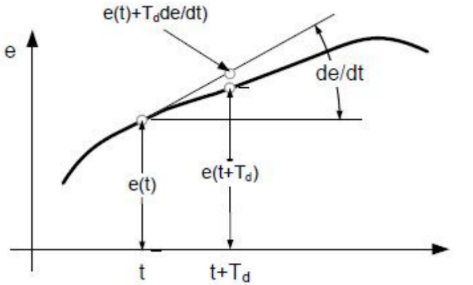
\includegraphics[width=0.3\linewidth]{el_8.png}
\centering
\caption{Диференцијално дејство како предвидувач на грешка}
\label{fig:el_8.png}
\end{figure}

\begin{figure}[H]
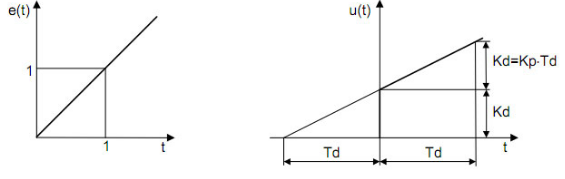
\includegraphics[width=0.3\linewidth]{el_9.png}
\centering
\caption{Дејствување на ПД регулатор}
\label{fig:el_9.png}
\end{figure}



\subsubsection{ПИД контролери во LabVIEW}

Прикажан подолу во сл.\ref{fig:PIDBlock.png} е блокот за ПИД контролер од Real Time модулот на LabVIEW. Првиот влез од левата страна е портата за грешка што функционира исто како и сите други кои досега се спомнати. Во следниот влез, наречен setpoint, се доведува референтната вредност кон која се стремиме, додека во process variable ја доведуваме големината која што ја управуваме. Следните 3 влезови одговараат на коефициентите на ПИД управувањето, односно пропорционалниот, интегралниот, и диференцијалниот коефициент соодветно.

Од десната страна имаме излез на грешката и излезот што одговара на самата управувана вредност.

\begin{figure}[H]
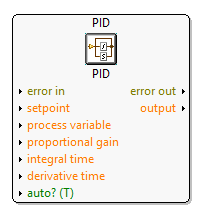
\includegraphics[width=0.3\linewidth]{PIDBlock.png}
\centering
\caption{LabVIEW ПИД Блок}
\label{fig:PIDBlock.png}
\end{figure}


\newpage

\section{Изработени Алгоритми}
Во текот на нашата работа со DaNI роботот, развивме 2 алгоритми за неговото управување. Првиот алгоритам имаше задача да го држи роботот на фиксно растојание од пречката (што се детектираше со ултразвучниот сензор), додека вториот алгоритам беше изработен со цел да се изедначат брзините на двете тркала. Двата алгоритми се базираат на управување со повратна врска, употребувајќи ПД контролери. Третиот алгоритам е примерниот алгоритам за избегнување на пречки даден од NI за демонстрација.

\subsection{Одржување на фиксно растојание со ПД контролер}
%Just a text based description of what's happening on the printout of the program, given by nikola. 
%Start at sensor feedback loop. Explain signal processing and clipping/tolerances. Runs into PID.
%Feed speed into motors, ezpz. 
Овој алгоритам ја има задачата да го одржи роботот на фиксно растојание од некоја детектирана пречка. Ова го постигнува со помош на ултразвучниот сензор на DaNI, VI-та дадени од NI Robotics модулот, и еден од вградените ПИД контролери во LabVIEW.\\ Алгоритамот ќе биде постепено образложен во продолжение:

\begin{enumerate}
\item Започнувајќи од левата страна, најпрво се повикува блокот за инцијализација (сл.\ref{fig:init.png}). На влез се доведува IP адресата на роботот, кој служи за идентификација на истиот. Како излез на овој блок се добива „објектот“ што го претставува DaNI, и секој од блоковите кој има било какво заемнодејство со роботот мора да прима копија од овој објект.
\item Се повикува блокот за насочување на сензорот (сл.\ref{fig:write_servo.png}) да осигури дека ултразвучниот сензор е насочен токму право пред роботот.
\item Следно алгоритамот влегува во \textit{while} циклус. Во овој \textit{while} циклус се отчитува растојанието од сензорот до пречката со \textit{Read Ping)))} блокот (сл.\ref{fig:read_ping.png}).
\item Ова отчитано растојаниe се заокружува во нашиот VI - \textit{dp.vi}, кој како влез го прима бројот што се заокружува и бројот на посакани децимални места.
\item Овој заокружен број се доведува до влезот на ПИД контролерот како управувана вредност (process variable). Забелешка: Во нашиот случај И терминот на ПИД-от не се употребува, односно работиме со ПД управување.
\item На влезовите на ПИД-от за пропорционално засилување и диференцијално засилување се доведуваат експериментално одредените константи
\item Излезната вредност од ПИД контролерот се зема како да е брзина во $m/s$, и се употребува за управување на моторите. Се заокружува на сличен начин употреубајќи го \textit{dp.vi}.
\item Заокружената брзина се доведува во влезовите на соодветниот блок (сл.\ref{fig:write_dc.png}). Како што е и претходно наведено, брзината што се доведува до левото тркало мора да се негира.
\item При STOP сигнал, \textit{while} циклусот завршува, и брзината на моторите се подесува на 0.
\item Алгоритамот чека 500ms пред да го повика финалниот блок за деиницијализација (сл.\ref{fig:deinit.png}).
\end{enumerate}

\begin{figure}[H]
\centering
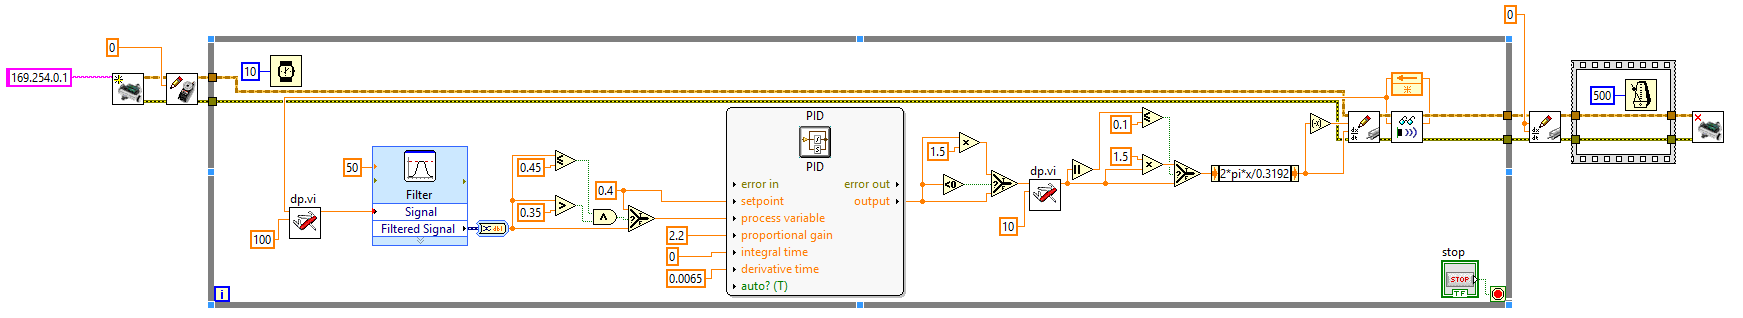
\includegraphics[width=0.80\paperheight,angle=90]{PID_Control.png}
\caption{Алгоритамот за одржување на растојание}
\label{fig:PID_Control.png}
\end{figure}

\subsection{Компензација на брзинска грешка со ПД контролер}

Поради разлики во конструкцијата на моторите настанати за време на производство (што е честа појава кај сериско производство каде се зголемува квантитет и намалува цената, по сметка на квалитетот), помеѓу нив има мали разлики во работата. Т.е. еден од моторите реагира/работи побрзо од другиот. Заради ова изработивме алгоритам кој што прави компензација на брзината на еден од моторите во зависност од другиот. Кој мотор се зема за примерок (главен мотор) зависи од нас, и со користење на вградените енкодери и повратна врска со ПИД контролер, се врши изедначување на брзините. Во главно се користат истите елементи од претходниот алгоритам.\\ Алгоритамот ќе биде постепено образложен во продолжение:

\begin{enumerate}
\item Кога успешно ќе се воспостави контакт со уредот, вредноста на подесувачот на брзина на Front Panel-от се ресетира на default вредност од 0. Пред започнување на програмата исто така ги подесуваме посакуваните вредности на променливите за ПД контролерот.
\item Следно влегуваме во првиот \textit{while} циклус, каде што ја подесуваме посакуваната брзина на моторите, и таа ја впишуваме во нив со користење на \textit{Write DC} блокот. 
\item Во овој циклус помеѓу секоја итерација има пауза од $50ms$ и со \textit{Visible} блоковите, од Front Panel-от ги тргаме засега непотребните стоп копчиња, кои се појавуваат кога има потреба од нив.
\item Следно алгоритамот влегува во \textit{case structure} циклус каде што избираме кое тркало го избираме за главно, односно „погонско“ а кое ќе биде компензирано. Кога сме задоволни со изборот, притискаме \textit{Start Wheel Control} копчето и влегуваме во внатрешниот \textit{while} циклус. 
\item Во овој циклус се отчитуваат вредностите од енкодерите со \textit{Read DC} блокот (сл.\ref{fig:read_dc.png}).
\item Овие отчитани вредности влегуваат во ПИД контролерот, и во зависност од кое тркало ни е избрано за главно, тие влегуваат во обратни влезови во контролерот. Пример: Кога избираме десното тркало да е главно, неговата отчитана вредност ја внесуваме во \textit{Setpoint} влезот, а вредноста на левото тркало влегува во \textit{Process Variable}. Во обратен случај, т.е. кога левото тркало е избрано за главно, влезовите се обратни.
\item Излезот од ПИД контролерот го впишуваме во тркалото кое што го контролираме/компензираме. Бидејќи вредноста на излезот од ПИД контролерот е само грешката, таа мора да ја додадеме/одземеме од вредноста која што ја отчитуваме од самото тркало. За впишување на брзината во моторот го користиме \textit{Write DC} блокот (сл.\ref{fig:write_dc.png}).
\item Со притискање на END копчето (т.е. \textit{stop 2} сигнал), внатрешниот \textit{while} циклус завршува, и брзината на моторите се подесува на 0.
\item Алгоритамот чека 2000ms пред да го повика финалниот блок за деиницијализација (сл.\ref{fig:deinit.png}).
\end{enumerate}

\begin{figure}[H]
\centering
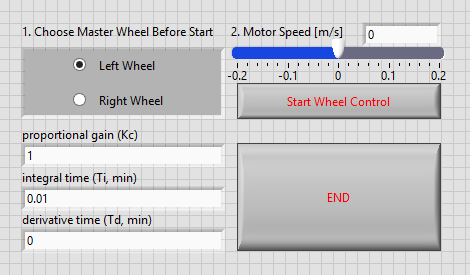
\includegraphics[width=0.75\linewidth]{wheel_control_fp.png}
\caption{Front Panel на алгоритамот за компензација на брзинска грешка}
\label{fig:wheel_control_fp.png}
\end{figure}

\begin{figure}[H]
\centering
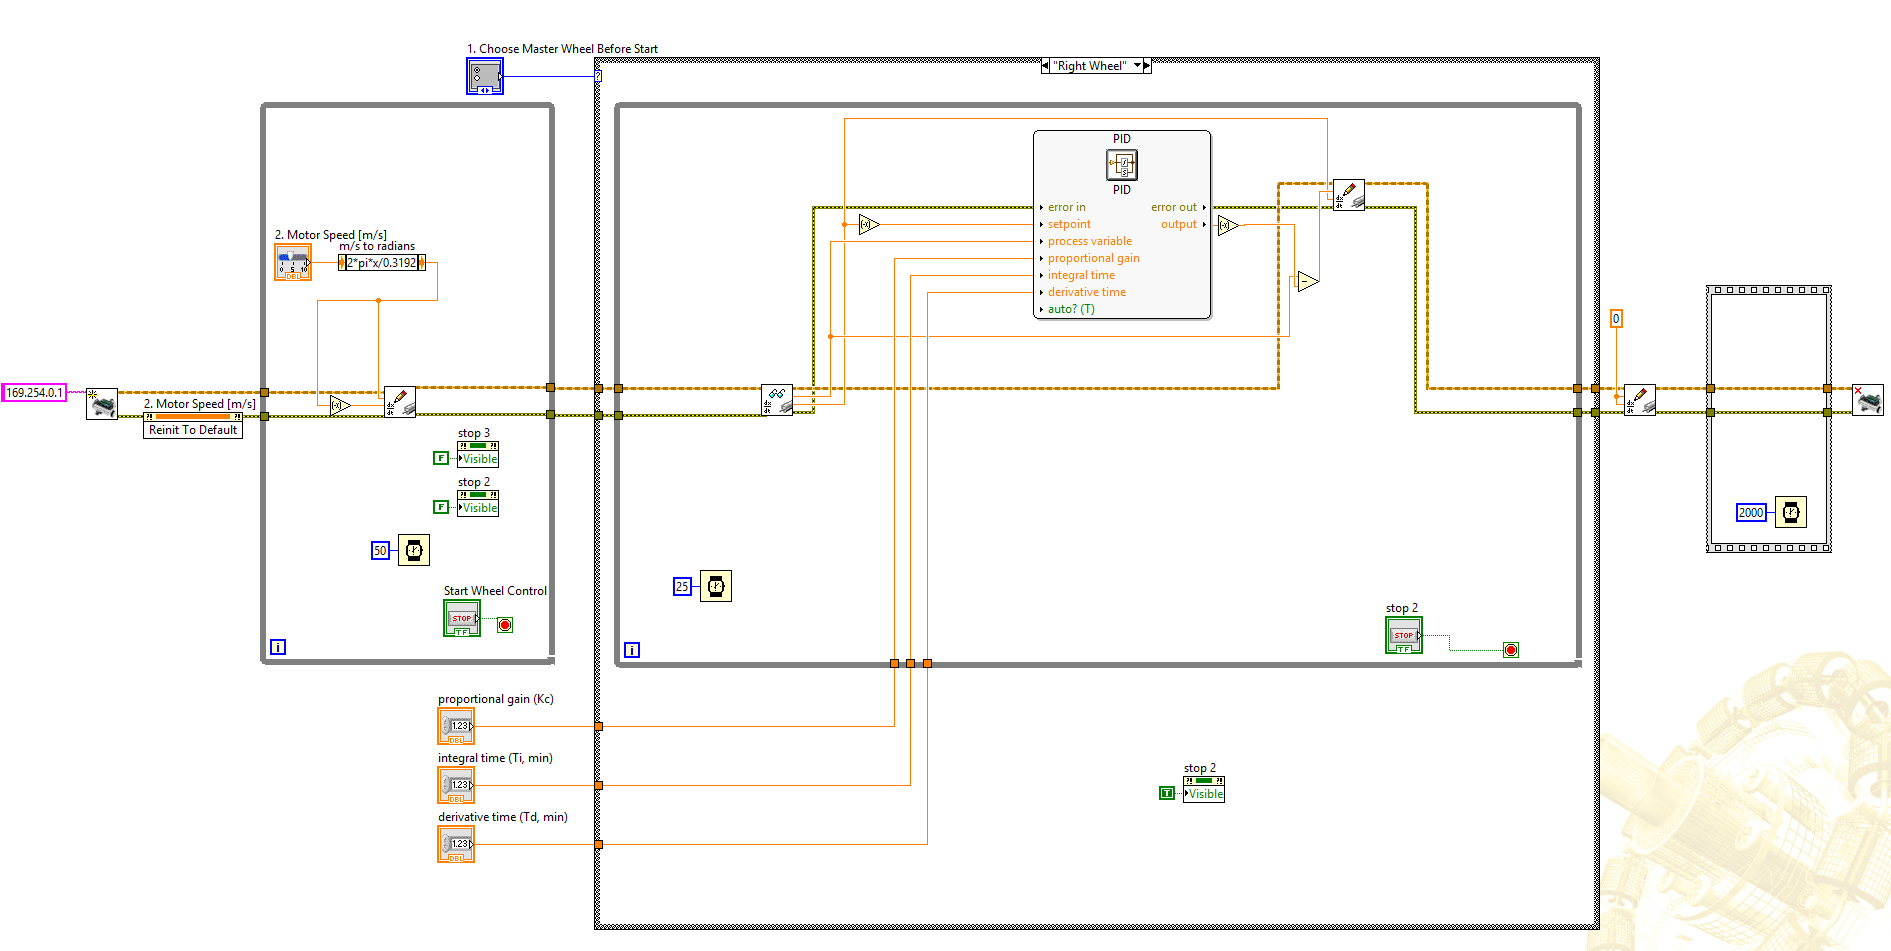
\includegraphics[width=0.75\paperheight,angle=90]{wheel_control_vi.png}
\caption{Алгоритамот за компензација на брзинска грешка}
\label{fig:wheel_control_vi.png}
\end{figure}

%Just a proof of concept PID link between left motor and right motor. One will be the setpoint giver, the other will follow and be
%controlled by the PID. Speeds should match up.

\subsection{Избегнување пречки со хистограм на векторски-полиња}
%OH BOY. This one will be a team effort.
Методот на хистограм со векторски полиња (ХВП) се состои од намалување (кратење) на податоци во две фази, наспроти постарите техники кои користат само еден чекор во кратење на податоци. Постојат три нивоа на претставување на податоци:
\begin{enumerate}
    \item Највисокото ниво содржи детален опис за околината во која се наоѓа роботот. Во ова ниво, дво-димензионалниот Cartesian хистограм (С) се надополнува со нови податоци во реално време. 
    \item Второто, средишно ниво е едно димензионален поларен хистограм (Н) кој се гради околу моменталната локација на роботот. Н содржи n аголни сектори со одредена ширина. 
    \item Последното ниво, најниското ниво, од претставување на податоци е излезот од ХВП алгоритамот.
\end{enumerate}

За разлика од другите програми, имплементацијата на ХВП во LabVIEW користи само локален поларен хистограм, а не и Cartesian хистограмот. Овој недостаток е исправен со вградување на енкодерот од кој што се црпат информации за далечина и правец. Поради што ние ќе се задржиме само на локалниот поларен хистограм.

Најпрво се генерира дво-димензионален хистограм околу роботот, што ги претставуваат пречките, чии што информации се добиваат од сензорот. Вториот чекор е конверзијата на дво -димензионалниот во едно-димензионален хистограм и потоа во поларен хистограм. Најпосле, алгоритамот го означува најдобриот сектор со ниски поларни вредности, и ги пресметува аголот и брзината во тој правец.

\begin{figure}[H]
\centering
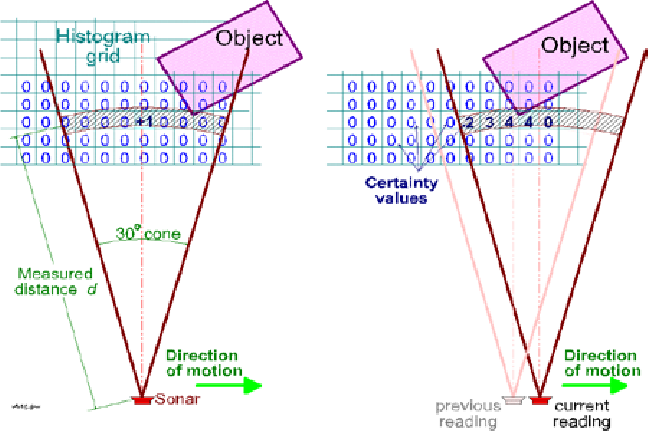
\includegraphics[width=0.35\linewidth]{2d_his.png}
\caption{Конструкција на 2D хистограм}
\label{fig:2d_his.png}
\end{figure}

\begin{figure}[H]
\centering
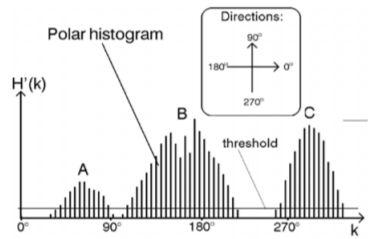
\includegraphics[width=0.35\linewidth]{1d_his.png}
\caption{Репрезентација на 1D хистограм}
\label{fig:1d_his.png}
\end{figure}

Принципот на работа е всушност избирање најголема празнина преку податоците од поларниот хисторграм, од каде што се пресметуваат правецот, насоката и оддалеченоста.

\begin{figure}[H]
\centering
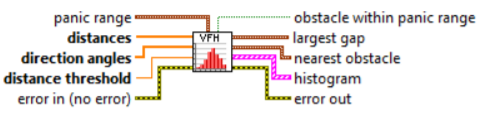
\includegraphics[width=0.5\linewidth]{vfh_lv.png}
\caption{ХВП блок во LabVIEW}
\label{fig:vfh_lv.png}
\end{figure}

Distances и direction angles се влезови кои што се добиваат од податоците кои што ги отчитува сензорот. Distances е низа од податоци за далечините на пречките. Direction angles аналогно е низа со агли кои што започнуваат од центарот на сензорот до секоја од далечините (аглите десно од центарот се означени како позитивни а оние лево од центарот како негативни вредности). Distance threshold е влез кој што дефинира пречки односно роботот игнорира објекти кои што се на далечина поголема од онаа на distance threshold. 
The nearest obstacle излез е структура од податоци која се добива како група од два елемента. ХВП дава излез на податоци на XY график. Блок дијаграмот на ХВП е даден на сл.\ref{fig:vfh_block_diagram.png}.

\begin{figure}[H]
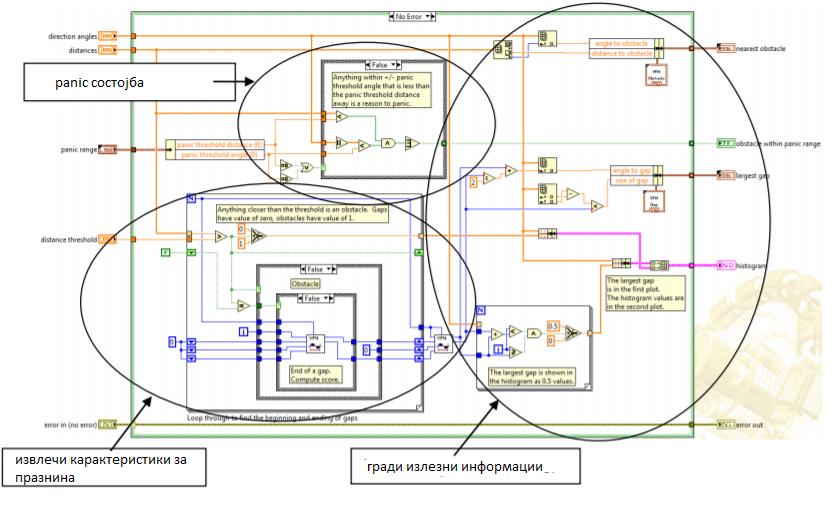
\includegraphics[width=0.75\linewidth]{vfh_block_diagram.png}
\centering
\caption{Блок дијаграм на Алгоритам за Избегнување}
\label{fig:vfh_block_diagram.png}
\end{figure}


За да се одреди дали одредена далечина претставува празнина или пречка, секој елемент се става во loop со индексирање при што се врши споредба со distance threshold. Имаме булов излез (1 или 0) при што 0 се доделува на далечини кои што се поголеми од distance threshold, а 1 доколку не се. Резултатот е низа со нули и единици кој што се менува како што роботот се движи. Компарацијата на излез е влез во Case Structure. Ако вредноста на моменталната празнина е подобра од минатата, се јавува true case, ако е обратно добиваме false case каде што претходните податоци на големина и офсет (реден број на вредноста во низа) се најдобра празнина и се сеуште излез.

%\section{Предизвици}

\section{Заклучок}
DaNi 2.0 нуди безброј можности преку кои не само што може да се совлада програмскиот јазик LabVIEW туку и да се разбере начинот на управување и користење на DC моторите и разни сензори. DaNi претставува темел (основа) за надоградба во покомплексни проекти кои би биле компетативни на брзиот раст на технолошки пронајдоци. Работата на овој проект беше ново искуство за сите нас како и голем предизвик да совладаме нов програмски јазик и да испрограмираме робот во толку кус рок. Секако работата на овој проект пред се беше и големо задоволство поаѓајќи од фактот што научивме многу нови нешта, се запознавме со покомплексен вид на применета математика (хистограм на векторски полиња), практично го применивме ПИД контролерот и имавме прилика вистински да програмираме во LabVIEW и успешно да направиме две различни програми на овој робот. Конечно, работата на овој проект ни пружи големо знаење кое што ќе можеме да го искористиме во иднината, а воедно беше и забавно.

\section{Понатамошна работа}
Употребувајќи го тоа што ги имаме научено од проектот, ќе продолжиме од тука да развиеме алгоритам за DaNI што ќе го оспособи прецизно да следи луѓе со помош на фузија на повеќе сензори, како камери и инфра-црвени низи. Можно проширување исто претставува додатокот на уште една камера што ќе може да препознава линии од разни бои, и да ја следи соодветната според изборот на корисникот.

\medskip
\nocite{*}
\printbibliography[heading=bibintoc,title={Користена литература}]

\end{document}


